% shared/template.tex
%
% Contiene un modello di documento che deve essere copiato e opportunamente
% modificato per creare i documenti 'concreti' di progetto. Definisce le macro
% specifiche per il documento corrente, importa la parte di preambolo condivisa
% e le pagine comuni a tutti i documenti.
% In particolare, per ogni documento concreto occorre per prima cosa aggiornare
% le macro, inserire una voce nella tabella delle modifiche e inserire il testo
% (o includere file sorgenti esterni) a partire dalla riga 66 in poi.

% **************************************************
% Macro specifiche per il documento corrente
% **************************************************
% Nome
\newcommand{\docName}{Piano di Progetto}
% Nome file
\newcommand{\docFileName}{piano di progetto}
% Versione
\newcommand{\docVers}{1.0}
% Data creazione
\newcommand{\creationDate}{05/12/2012}
% Data ultima modifica
\newcommand{\modificationDate}{06/12/2012}
% Stato in {Approvato, Non approvato}
\newcommand{\docState}{Non approvato}
% Uso in {Interno, Esterno}
\newcommand{\docUsage}{Interno}
% Redattori da specificare come nome1\\ &nome2\\ ecc.
\newcommand{\docAuthors}{Stefano Farronato\\ &Elena Zecchinato}
% Approvato da
\newcommand{\approvedBy}{}
% Verificatori
\newcommand{\verifiedBy}{}
% Perscorso (relativo o assoluto) che punta alla directory contenente shared/
% come sua sottodirectory (per comodità chiamiamola 'doc root').
\newcommand{\docRoot}{..}
\def\INDICETABELLE{true}
\def\INDICEFIGURE{true}

% importa il preambolo condiviso da tutti i documenti
% shared/preamble.tex
%
% Questo documento contiene la parte del preambolo condivisa e viene pertanto
% richiamato nel 'master' di tutti i documenti di progetto.  Al suo interno
% contiene le inclusioni (e le configurazioni) di tutti i package richiesti per
% la compilazione dei documenti, le macro di carattere generale e la definizione
% degli stili di pagina.

\documentclass[a4paper,10pt,openright]{article}

% **************************************************
% Macro generiche
% **************************************************
\newcommand{\team}{Software Synthesis}                    % chi siamo
\newcommand{\email}{software.synthesis@gmail.com}         % e-mail
\newcommand{\caName}{}                                    % titolo capitolato
\newcommand{\caDescr}{}                                   % descrizione
\newcommand{\inglese}[1]{\textit{#1}}

% **************************************************
% Codifica e lingua dei documenti
% **************************************************
\usepackage[utf8x]{inputenc}                              % codifica caratteri dei documenti sorgenti
\usepackage[english,italian]{babel}                       % localizzazione ai fini di sillabazione e cross-references
\usepackage[T1]{fontenc}                                  % codifica font di output

% **************************************************
% Definizione geometria della pagina
% **************************************************
\usepackage[a4paper,head=4cm,top=4.5cm,bottom=3cm,left=3cm,right=3cm,bindingoffset=5mm]{geometry}

% *************************************************
% Intestazioni e piè di pagina personalizzati
% *************************************************
\usepackage{fancyhdr}
% stile normale
\fancypagestyle{normal}{
\fancyhead{}                                              % intestazione
\fancyhead[RE,RO]{
\begin{picture}(0,0)
  \put(-410,0){
\includegraphics[width=1.02\textwidth]{header_logo}}
  \put(-410,10){\sffamily\large\leftmark}
\end{picture}
\vspace{-4pt}
}
\renewcommand{\headrulewidth}{.4pt}                       % riga sotto l'intestazione
\cfoot{}                                                  % piè di pagina
\fancyfoot[RO,LE]{\sffamily
  pag.~\thepage{} di \pageref{LastPage}}                  % a dx nelle pag. dispari e a sx in quelle pari
\fancyfoot[RE,LO]{\sffamily\docFileName{} -- v.\docVers}
\renewcommand{\footrulewidth}{.4pt}                       % riga sopra il piè di pagina
}
% stile per gli indici
\fancypagestyle{toc}{
\fancyhead{}                                              % intestazione
\fancyhead[RE,RO]{
\begin{picture}(0,0)
  \put(-410,0){
\includegraphics[width=1.02\textwidth]{header_logo}}
\end{picture}
}
\renewcommand{\headrule}{}                                % nessuna riga sotto l'intestazione
\cfoot{}                                                  % piè di pagina
\fancyfoot[RO,LE]{\sffamily\thepage{}}                    % a dx nelle pag. dispari e a sx in quelle pari
\fancyfoot[RE,LO]{\sffamily\docFileName{} -- v.\docVers}
\renewcommand{\footrulewidth}{.4pt}                       % riga sopra il piè di pagina
}

\pagestyle{fancy}                                         % premetto: non so usare bene le marche:
\renewcommand{\sectionmark}[1]{\markboth{#1}{#1}}         % se qualcuno ha idee migliori si faccia avanti!

% **************************************************
% Tabelle
% **************************************************
\usepackage{tabularx}                                     % tabelle di larghezza fissa con una o più colonne variabili
\usepackage{multirow}                                     % colonne con colonne che si estendono per più righe
\usepackage{booktabs}                                     % per inserire l'ambiente table e le righe orizz. nelle tabelle
\usepackage{longtable}			                          % tabelle oltre i limiti di pagina

% **************************************************
% Cross-references e collegamenti ipertestuali
% **************************************************
\usepackage[hidelinks]{hyperref}
\hypersetup{%
  colorlinks=false, linktocpage=false, pdfborder={0,0,0}, pdfstartpage=3, pdfstartview=FitV,%
  urlcolor=Cyan, linkcolor=Cyan, citecolor=Black, %pagecolor=Black,%
  pdftitle={\docName}, pdfauthor={\team}, pdfsubject={}, pdfkeywords={},%
  pdfcreator={pdflatex}, pdfproducer={pdflatex with hyperref package}%
}

% **************************************************
% Immagini e grafica
% **************************************************
\usepackage{graphicx}                                     % supporto ad aspetti avanzati delle immagini
\graphicspath{{\docRoot/pics/}}                           % percorso contenente tutti i file immagini
\usepackage{color}                                        % permette di colorare facilmente il testo

% **************************************************
% Altri pacchetti opzionali
% **************************************************     
\usepackage{lastpage}                                     % per sapere il numero totale di pagine
\usepackage{lipsum}                                       % genera "dummy text" per prove di impaginazione
\usepackage{eurosym}                                      % per il simbolo dell'euro usare \EUR{x} dove x è l'importo


% Fine del preambolo e inizio del documento
\begin{document}

% Inclusione della prima pagina
% shared/firstpage.tex
%
% Questo documento definisce il contenuto della prima pagina, che si suppone
% essere uguale in tutti i documenti.  Oltre al logo e al titolo, la prima
% pagina contiene i metadati relativi al documento in cui viene inclusa.


% rimuove intestazioni e piè di pagina
\pagestyle{empty}

\begin{center}

% logo del gruppo

\includegraphics[width=1.5\textwidth]{logo}

\vspace{1in}

% titolo del documento
{\Huge\bfseries \docName}

\vspace{1in}

% tabella riepilogativa
\begin{tabularx}{.7\textwidth}{>{\bfseries\sffamily}l>{\sffamily}l}
\toprule
\multicolumn{2}{>{\sffamily}c}{Informazioni sul documento}\\
\midrule
Nome file:            & \docFileName\\
Versione:             & \docVers\\
Data creazione:       & \creationDate\\
Data ultima modifica: & \modificationDate\\
Stato:                & \docState\\
Uso:                  & \docUsage\\
Redattori:            & \docAuthors\\
Approvato da:         & \approvedBy\\
Verificatori:         & \verifiedBy\\
\bottomrule
\end{tabularx}

\end{center}

\newpage


% Storico delle modifiche
\section*{Storia delle modifiche}
\begin{tabularx}{\textwidth}{lXll}
\toprule
Versione & Descrzione intervento & Redattore & Data\\
\midrule % inserire qui il contenuto della tabella
0.13 &Inserimento tabelle nella sezione "Preventivo", & Stefano Farronato & 12/12/2012\\
0.12 &Correzione contenuti nella sezione "Pianificazione", & Stefano Farronato & 12/12/2012\\
0.11 &Inserimento GANT, tabelle e immagini nella sezione "Pianificazione," & Stefano Farronato & 12/12/2012\\
0.11 &Stesura e analisi sezione "Verifica e Validazione", & Elena Zecchinato & 11/12/2012\\
0.10 &Stesura e analisi sezione "Progettazione di dettaglio e Codifica", & Stefano Farronato & 10/12/2012\\
0.9 &Stesura e analisi sezione "Progettazione Architetturale", & Stefano Farronato & 10/12/2012\\
0.8 &Stesura e analisi sezione "Analisi", "Ruoli e Costi" & Elena Zecchinato & 08/12/2012\\
0.7 &Stesura e analisi sezione "Pianificazione", "Analisi", "Ruoli e Costi" & Elena Zecchinato & 08/12/2012\\
0.6 &Stesura e analisi del "Modello di ciclo di vita", & Stefano Farronato & 06/12/2012\\
0.5 &Modifica sezione "analisi dei rischi" con introduzione e analisi di nuovi rischi, & Stefano Farronato & 06/12/2012\\
0.4 & Modifica sezione "analisi dei rischi" con introduzione e analisi di nuovi rischi, & Elena Zecchinato & 05/12/2012\\
0.3 & Stesura "Riferimenti", & Stefano Farronato & 05/12/2012\\
0.2 & Stesura "analisi dei rischi", & Stefano Farronato & 05/12/2012\\
0.1 & Stesura scheletro documento, introduzione e introduzione preliminare dei rischi & Stefano Farronato & 05/12/2012\\
\bottomrule
\end{tabularx}
\newpage

% inclusione dell'indice
% shared/toc.tex
%
% Questo file contiene le istruzioni che generano l'indice o gli indici del
% documento (utile nel caso in cui decidessimo di avere anche un indice delle
% tabelle e/o un indice delle figure).

\pagestyle{toc}
\pagenumbering{roman}

\tableofcontents

\newpage


% Alcuni aggiustamenti per le pagine
\pagenumbering{arabic}
\setcounter{page}{1}
\pagestyle{normal}

% Qui ha inizio il documento vero e proprio...
\section{Organigramma}

\section{Introduzione}
\subsection{Scopo del prodotto}
Con progetto "MyTalk" intendiamo un sistema software di comunicazione tra utenti mediante browser, utilizzando solo componenti standard, senza dover installare plugin o programmi esterni. L'utilizzatore dovrà poter chiamare un altro utente, iniziare la comunicazione sia audio che video, svolgere la chiamata e terminare la chiamata ottenendo delle statistiche sull'attività.

\subsection{Scopo del documento}
Il seguente documento ha lo scopo di presentare e definire i ruoli professionali dei membri del Team di lavoro dell'azienda Software Synthesis sul progetto "MyTalk" regolarmente accettato dall'azienda appaltatrice Zucchetti s.r.l.\\
Sono inoltre descritti i costi stimati necessari al completamento di tale progetto e i rischi possibili nella sua realizzazione.Infine viene stilato il carico di lavoro distribuito per ogni soggetto del Team mediante un organigramma specificante tempo e risorse.
\subsection{Glossario}
Al fine di evitare incomprensioni dovute all'uso di termini tecnici nei documenti, viene redatto e allegato il documento "Glossario.pdf" dove vengono definiti e descritti tutti i termini marcati con una sottolineatura.

\section{Riferimenti}
\subsection{Normativi}
VINCOLI DI ORGANIGRAMMA: Specificate dal Committente designato all'indirizzo\\ \textit{http://www.math.unipd.it/~tullio/IS-1/2012/Progetto/PD01b.html} \\\\
NORME DI PROGETTO  v1.0 allegato

\subsection{Informativi}
RIFERIMENTI INFORMATIVI
CAPITOLATO D'APPALTO: MyTalk, v 1.0, redatto e rilasciato dal proponente Zucchetti s.r.l reperibile all'indirizzo:\\ \textit{http://www.math.unipd.it/~tullio/IS-1/2012/Progetto/C1.pdf} \\\\
TESTO DI CONSULTAZIONE: Software Engineering (8th edition) Isan Sommerville, Pearson Education | Addison-Wesley


\section{Modello di ciclo di vita}
Per lo sviluppo del prodotto MyTalk, il Team di Software Synthesis ha optato per il modello di ciclo di vita incrementale. Questa scelta è stata dettata da scelte prevalentemente dettate dalla scarsa esperienza dell'azienda nello sviluppo di determinati progetti, nonchè la scelta di realizzare un prodotto mediante passi pianificati in modo da poter gestire l'intero svolgimento progettuale nei tempi e nei costi previsti.\\\\
Questo tipo di modello inoltre permetterà di sviluppare e completare il software sviluppando i requisiti minimi obbligatori imposti dal committente, procedendo successivamente all'integrazione dei requisiti facoltativi e desiderabili presi in considerazione. Si conclude quindi che il modello sarà dunque composto da due iterazioni.\\\\
Basandoci sulle specifiche dettate da questo tipo di modello, il Team svolgerà inizialmente (e una sola volta) le fasi di analisi e progettazione a livello architetturale ad alto livello, successivamente si lavorerà iterativamente sul controllo e la valutazione della realizzazione nel dettaglio.\\

\section{Pianificazione}
\subsubsection{Ruoli e Costi}
I ruoli  costituiscono delle funzioni aziendali che vengono assegnate al progetto.\\
La seguente tabella riporta i ruoli che devono essere ricoperti dai membi del Team e i rispettivi costi orari:
\begin{table}[h]
\centering
\begin{tabular}{|l|cl|}
\hline
Ruolo& Costo Orario&  \\
\hline
Responsabile & 30 euro &\\
Amministratore  & 20 euro&\\
Analista & 25 euro&\\
Progettista  & 22 euro&\\
Programmatore & 15 euro&\\
Verificatore & 15 euro&\\
\hline
\end{tabular}
\caption{costo orario per ruolo}
\end{table}\\
Al fine di permettere che ogni membro del gruppo posso ricoprire almeno una volta ogni ruolo, è necessario adottare un meccanismo di rotazione.\\
Tale meccanismo dovrà garantire, oltre alla rotazione, che non vi siano conflitti di interesse, ovvero che non ci siano periodi in cui una stessa risorsa sia verificatrice di se stessa.\\

\subsubsection{Analisi}
Questa fase inizia in data 29/11/2012 e finisce in data 10/01/2013.\\
Tuttavia la data di consegna dei documenti che descrivono le fasi d'analisi sono previste il giorno 21/12/2012, restringendo il tempo produttivo effettivo.\\
Questa fase coinvolge i ruoli di Responsabile, Amministratore, Analista e Verificatore.
Le ore svolte dai vari componenti in questa fase non rientrano nel preventivo, la fase di analisi costituisce infatti un investimento da parte dell’azienda e non può quindi essere a carico del proponente ne faranno parte del massimo complessivo finale di 100 ore lavorative per componente .
Verrà in ogni caso tenuto traccia del dettaglio delle ore compiute per la già concordata rotazione dei ruoli dei membri del Team.

\begin{figure}[h]
  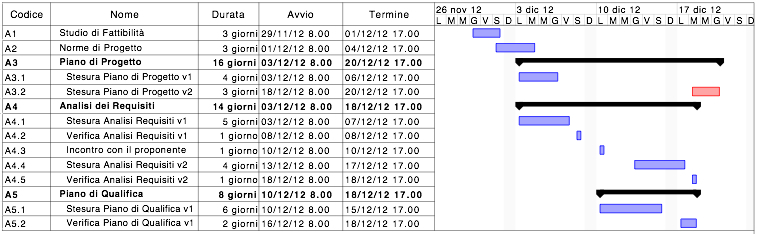
\includegraphics[width=\textwidth]{Analisi}
\caption{Gant della pianificazione d'Analisi }
\end{figure}

I ruoli sono in questa fase definiti come in tabella X:\\
\begin{table}[h]
\centering
\begin{tabular}{|l|c|c|c|c|c|cl|}
\hline
Componente& RE& AM& AN& PRO& PRG& VER& \\
\hline
Beraldin Diego & 2& & 8& & & 10&\\
Farronato Stefano & 8& 2& 10& & & &\\
Meneghinello Andrea & & 6& 15& & & &\\
Rizzi Andrea & & & 21& & & &\\
Schivo Marco & & 12& & & & 10&\\
Tresoldi Riccardo & & & 21& & & &\\
Zecchinato Elena & 10& & 10& & & &\\
\hline
Totale & 20& 20& 77& & & 20&\\
\hline
\end{tabular}
\caption{copertura ruoli nella fase di Analisi}
\end{table}\\

\begin{figure}[h]
  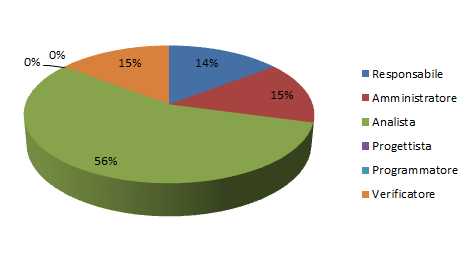
\includegraphics[width=\textwidth]{torta_analisi}
\caption{Torta ripartizione ruoli nella fase di Analisi}
\end{figure}

\begin{table}[h]
\centering
\begin{tabular}{|l|cl|}
\hline
Componente& Totale& \\
\hline
Beraldin Diego & 20&\\
Farronato Stefano & 20&\\
Meneghinello Andrea & 21&\\
Rizzi Andrea &  21&\\
Schivo Marco & 22&\\
Tresoldi Riccardo & 21&\\
Zecchinato Elena & 20&\\
\hline
\end{tabular}
\caption{copertura ruoli nella fase di Analisi}
\end{table}

\subsubsection{Progettazione Architetturale}
Questa fase inizia in data 09/01/2013 e finisce in data 31/01/2013, per un totale di 20 giorni lavorativi. \\
Questa fase coinvolge i ruoli di Responsabile, Amministratore, Analista, Progettista e Verificatore.
L'analista in questa fase avrà un ruolo prevalentemente rifinitorio (ma doveroso) nei confronti dell'Analisi dei Requisiti, per rendere più sicuro e corretto possibile l'avvio progettuale della Specifica Tecnica.
Si è deciso di suddividere questo periodo in due fasi. La prima fase termina il 16/01/2013 e ed inizia la seconda, di seguito la tabella con la pianificazione dei compiti:\\
\begin{figure}[h]
  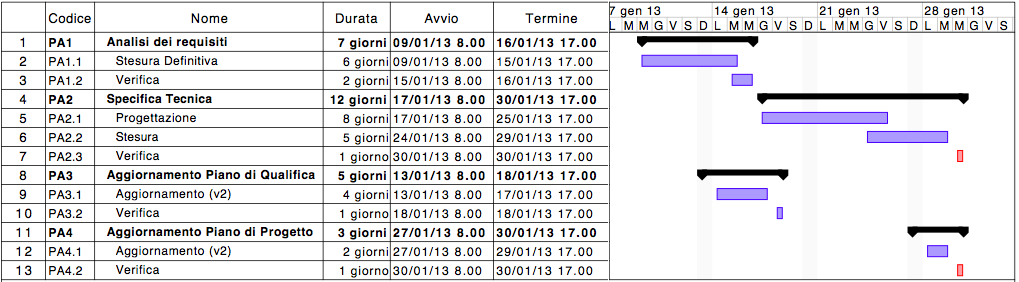
\includegraphics[width=\textwidth]{Progettazione_Architetturale}
\caption{Gant della Progettazione Architetturale }
\end{figure}\\
I ruoli sono in questa fase definiti come in tabella X:\\
\begin{table}[h]
\centering
\begin{tabular}{|l|c|c|c|c|c|c|c|cl|}
\hline
Componente& RE& AM& AN& PRO(fase1)& PRO(fase2)& PRG& VER(fase1)& VER(fase2)& \\
\hline
Beraldin Diego & & 8& 15& & 13& & & &\\
Farronato Stefano & & & & 22& & & & 16&\\
Meneghinello Andrea & 9& & & 12& & & & 13&\\
Rizzi Andrea & & 8& & & 16& & 16& &\\
Schivo Marco & & & 15& 20& & & & &\\
Tresoldi Riccardo & 7& & & 18& & & & 11&\\
Zecchinato Elena & & & & & 10& & 25& &\\
\hline
Totale & 16& 16& 30& 72& 39& & 41& 40&\\
\hline
\end{tabular}
\caption{copertura ruoli nella fase di Progettazione Architetturale}
\end{table}\\
Ad ogni risorsa sarà distribuito il seguente carico di lavoro (figura X):\\
\begin{figure}[h]
  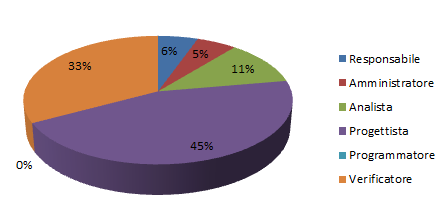
\includegraphics[width=\textwidth]{torta_PA}
\caption{Torta ripartizione ruoli nella fase di Progettazione Architetturale}
\end{figure}\\
Infine vengono fornite le ore distinte per componente del Team che sono state svolte in questa fase (tabella X):\\
\begin{table}[h]
\centering
\begin{tabular}{|l|c|c|cl|}
\hline
Componente& Fase I& Fase II& Totale& \\
\hline
Beraldin Diego &23 &13 & 36&\\
Farronato Stefano & 22& 16& 38&\\
Meneghinello Andrea & 21& 13& 34&\\
Rizzi Andrea & 16& 24& 40&\\
Schivo Marco & 20& 15& 35&\\
Tresoldi Riccardo & 18& 18& 36&\\
Zecchinato Elena & 25& 10& 35&\\
\hline
\end{tabular}
\caption{copertura ruoli nella fase di progettazione architetturale}
\end{table}


\subsubsection{Progettazione di Dettaglio e Codifica}
La seguente fase inizia in data 07/02/2013 e terminerà in data 06/03/2013. In questo periodo si svilupperà la progettazione di dettaglio del prodotto MyTalk e la sua codifica.
In questa fase, coerentemente con il modello di ciclo di vita scelto, la fase di Progettazione di Dettaglio e la Codifica avverranno per iterazioni.
Sono previste X iterazioni, al terimine della prima sarà possibile avere il primo prototipo per testare le funzioni di MyTalk, in data 22/03/2013.
E' stata scelta tale data anche per provvedere ad una doverosa rotazione di ruoli all'interno del Team di sviluppo, per consentire a tutti i soggetti di raggiungere il massimo apprendimento pratico dei vari compiti.
Il diagramma di Gantt in figura X descrive l'organizzazione lavorativa:\\

\begin{figure}[h]
  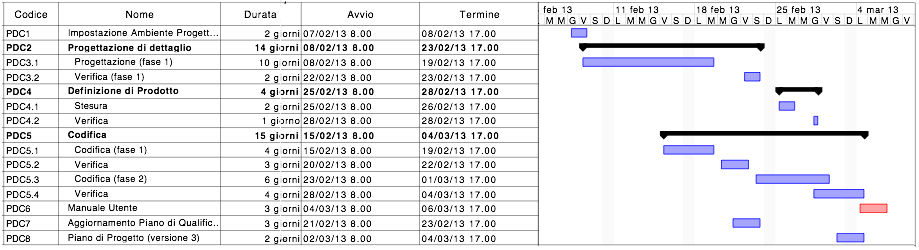
\includegraphics[width=\textwidth]{Progettazione_di_Dettaglio_e_Codifica}
\caption{Gant della Progettazione di Dettaglio e Codifica}
\end{figure}


I ruoli sono in questa fase definiti come in tabella X:\\
\begin{table}[h]
\centering
\begin{tabular}{|l|c|c|c|c|c|c|c|cl|}
\hline
Componente& RE& AM& AN& PRO& PRG(fase1)&VER(fase1)& PRG(fase2)& VER(fase2)& \\
\hline
Beraldin Diego & & & & & 24& & & 23&\\
Farronato Stefano & & & & 15&14 & & & 18&\\
Meneghinello Andrea & & & & & & 25& 19& &\\
Rizzi Andrea & 9& & & 22& & & 12& &\\
Schivo Marco & & & & 16& 10& & & 20&\\
Tresoldi Riccardo & & 7& & & & 20& 20& &\\
Zecchinato Elena & & & & 25& & & 20& &\\
\hline
Totale & 9& 7& 0& 78& 48& 45& 71& 61&\\
\hline
\end{tabular}
\caption{copertura ruoli nella fase di Progettazione di Dettaglio e Codifica}
\end{table}
\\\\
Ad ogni risorsa sarà distribuito il seguente carico di lavoro (figura X):\\
\begin{figure}[h]
  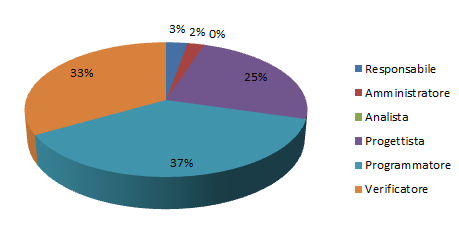
\includegraphics[width=\textwidth]{torta_PDC}
\caption{Torta ripartizione ruoli nella fase di Progettazione di Dettaglio e Codifica}
\end{figure}
\\\\
Infine vengono fornite le ore distinte per componente del Team che sono state svolte in questa fase (tabella X):\\
\begin{table}[h]
\centering
\begin{tabular}{|l|c|c|cl|}
\hline
Componente& Fase I& Fase II& Totale& \\
\hline
Beraldin Diego & 24& 23& 47&\\
Farronato Stefano & 29& 18& 47&\\
Meneghinello Andrea & 26& 20& 44&\\
Rizzi Andrea &31 &12 & 43&\\
Schivo Marco & 26& 20& 46&\\
Tresoldi Riccardo & 27& 20& 47&\\
Zecchinato Elena & 25& 20& 45&\\
\hline
\end{tabular}
\caption{copertura ruoli nella fase di progettazione di dettaglio e codifica}
\end{table}

\subsubsection{Verifica e Validazione}
Questa fase inizia in data 05/03/2012 e finisce in data 22/03/2012, per un totale di 16 giorni lavorativi.
Questa fase coinvolge i ruoli di Responsabile, Amministratore, Progettista, Programmatore e Verificatore. Si può notare che non è più attivo quindi il ruolo di Analista, si prevede infatti che la in questa fase l’attività di analisi sia ovviamente conclusa.
Si è deciso di inserire  in questo periodo anche il ruolo del programmatore in quanto di prevede che qualche ora di programmazione potrebbe essere necessaria al fine di terminare lo sviluppo del software iniziato nelle fasi precedenti.
In oltre non si è ritenuta necessaria la suddivisione in fasi del periodo visto che le attività riguardano in gran parte il processo di verifica e validazione e quindi non vi è la necessità di una forte rotazione.
Essendoci però la presenza dei ruoli di Progettista e Programmatore per un numero limitato di ore e la necessità di impiegare risorse nel ruolo di Verificatore, sarà necessario impiegare le persone che svolgono tali ruoli nelle attività di verifica e validazione.  
Nell’assegnazione dei ruoli si è volta particolare attenzione al conflitto di interessi,  progettando una distribuzione tale da evitare la situazione surreale in cui un verificatore controlli il suo stesso operato.\\
Il diagramma di Gantt in figura X descrive l'organizzazione lavorativa:\\
\begin{figure}[h]
  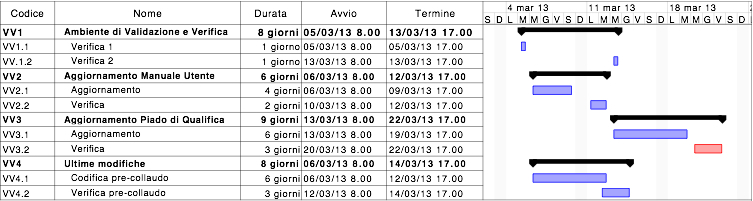
\includegraphics[width=\textwidth]{Verifica_e_Validazione}
\caption{Gant della Verifica e della Validazione}
\end{figure}
I ruoli sono in questa fase definiti come in tabella X:\\
\begin{table}[h]
\centering
\begin{tabular}{|l|c|c|c|c|c|cl|}
\hline
Componente& RE& AM& AN& PRO& PRG& VER& \\
\hline
Beraldin Diego & & & & & & 20&\\
Farronato Stefano & & & & & 5& 18&\\
Meneghinello Andrea & & & & 5& & 15&\\
Rizzi Andrea & & & & & & 20&\\
Schivo Marco & 6& & & & & 16&\\
Tresoldi Riccardo & & & & & & 20&\\
Zecchinato Elena & & 8& & & & 15&\\
\hline
Totale & 6& 8& 0& 5& 5& 124&\\
\hline
\end{tabular}
\caption{copertura ruoli nella fase di Verifica e Validazione}
\end{table}
\\\\
Ad ogni risorsa sarà distribuito il seguente carico di lavoro (figura X):\\
\begin{figure}[h]
  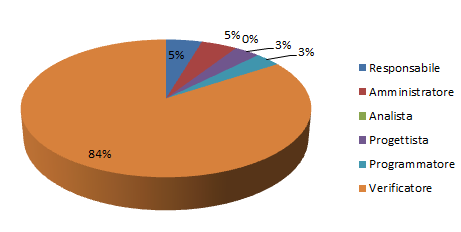
\includegraphics[width=\textwidth]{torta_VV}
\caption{Torta ripartizione ruoli nella fase di Verifica e Validazione}
\end{figure}
\\\\
Infine vengono fornite le ore distinte per componente del Team che sono state svolte in questa fase (tabella X):\\
\begin{table}[h]
\centering
\begin{tabular}{|l|cl|}
\hline
Componente& Totale& \\
\hline
Beraldin Diego & 20&\\
Farronato Stefano & 23&\\
Meneghinello Andrea & 20&\\
Rizzi Andrea & 20&\\
Schivo Marco & 22&\\
Tresoldi Riccardo & 20&\\
Zecchinato Elena & 23&\\
\hline
\end{tabular}
\caption{copertura ruoli nella fase di Verifica e Validazione}
\end{table}

\section{Preventivo}
\subsubsection{Prospetto Orario}
La tabella 10 illustra le ore totali di lavoro produttivo di ciascun membro del team Software Synthesis, per soggetto è stato preventivato un totale di 103 ore produttive, pertanto coerenti con le richieste vincolanti.
\begin{table}[h]
\centering
\begin{tabular}{|l|c|c|c|c|c|c|cl|}
\hline
Componente& RE& AM& AN& PRO& PRG& VER& TOTALE&\\
\hline
Beraldin Diego & A& 8& 15& 13& 24& 43& 103&\\
Farronato Stefano & A& A& A& 37& 14& 52&  103&\\
Meneghinello Andrea & 9& A& A& 17& 24& 53& 103&\\
Rizzi Andrea & 9& 8& A& 38& 12& 36& 103&\\
Schivo Marco & 6& A& 15& 36& 10& 36& 103&\\
Tresoldi Riccardo & 7& 7& A& 18& 20& 51& 103&\\
Zecchinato Elena & A& 8& A& 35& 20& 40& 103&\\
\hline
\end{tabular}
\caption{Dettaglio delle ore totali preventivate}
\end{table}

Ad ogni risorsa sarà distribuito il seguente carico di lavoro per portare a compimento il Progetto MyTalk (figura X):\\
\begin{figure}[h]
  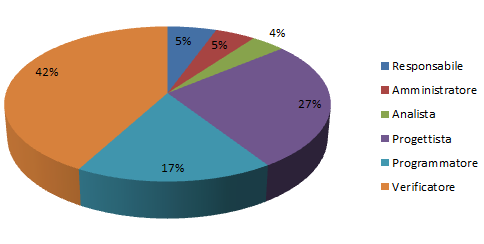
\includegraphics[width=\textwidth]{torta_totale}
\caption{Torta ripartizione ruoli in tutto il periodo di svolgimento del Progetto MyTalk}
\end{figure}
\\\\

\subsubsection{Prospetto Economico}
Il Progetto nella sua realizzazione avrà un costo stimato calcolato nella tabella 11 di seguito esposta, anche in questo caso il progetto impone un impegno economico coerente con i parametri imposti da capitolato.
\begin{table}[h]
\centering
\begin{tabular}{|l|c|cl|}
\hline
Ruolo& Ore& Costo& \\
\hline
Responsabile & 31 & 930 euro&\\
Amministratore  & 31& 620 euro&\\
Analista & 30& 750 euro&\\
Progettista  & 194& 4268 euro&\\
Programmatore & 124& 1860 euro&\\
Verificatore & 311 & 4665 euro&\\
\hline
Totale & 721 &13.093,00 euro&\\
\hline
\end{tabular}
\caption{costo e ore per ogni ruolo di progetto}
\end{table}

\section{Analisi dei rischi}
In questa sezione vengono analizzati in modo mirato e approfondito i rischi che abbiamo individuato come possibili durante lo svolgimento del progetto. L'individuazione e la strategia di gestione di tali rischi è fondamentale per la pianificazione delle fasi di lavoro e la loro corretta esecuzione.\\
Infatti solo tramite un approccio di gestione ai fattori di rischio è possibile tutelarsi dalla loro eventuale insorgenza e mitigarne gli effetti.\\
Data la scarsa esperienza del Team su tali tematiche, il gruppo si è affidato a delle (una?) sessioni/e di brain-storming collettiva/e cercando di focalizzare i vari punti critici. \\\\
Per rendere efficace l'analisi di ogni rischio si è deciso di quantificarlo mediante un apposita scala di valutazione sia dal punto di vista della probabilità che il rischio si manifesti (livello), sia il suo grado di incidenza sul progetto stesso (impatto):\\\\
\begin{table}[h]
\centering
\begin{tabular}{|l|cl|}
\hline
Probabilità& Descrizione&  \\
\hline
ALTA & probabilità elevata che si verifichi&\\
MEDIA & probabilità equivalente nel verificarsi o meno&\\
BASSA & pprobabilità bassa che si verifichi&\\
\hline
\end{tabular}
\caption{Probabilità e Descrizione probabilità di un rischio}
\end{table}
\\\\
\begin{table}[h]
\centering
\begin{tabular}{|c|cl|}
\hline
Scala& Descrizione&  \\
\hline
5 & conseguenze molto gravi&\\
4 & conseguenze gravi&\\
3 & conseguenze medio-gravi&\\
2 & conseguenze minimali&\\
1 & nessuna/lievi conseguenze&\\
\hline
\end{tabular}
\caption{Scala e descrizione delle conseguenze di un rischio}
\end{table}

\subsection{Rischi di Progetto}
\subsubsection{Problemi personale}
\begin{description}
	\item{\scshape\bfseries Analisi:} durante la realizzazione del progetto è probabile che alcuni membri del Team siano soggetti a problemi fisiologici e/o sovvengano impegni personali improrogabili che porteranno ad una sicura modifica della pianificazione del lavoro collettivo. L'impatto di tale rischio è variabile in base al soggetto mancante, in quanto può essere assegnato ad un'attività (o ruolo) più o meno importante all'interno del progetto.
	\item{\scshape\bfseries Probabilità:} ALTA
	\item{\scshape\bfseries Impatto:} variabile
	\item{\scshape\bfseries Strategia di Gestione:}per mitigare gli effetti di tali fenomeni è ragionevole prima di tutto pianificare i tempi di lavoro personali in modo da lasciare un lasco di tempo tra un attività e l'altra. Così facendo la gestione temporale (compresa di eventuali imprevisti) risulta meno incline a modifiche e/o modifiche dei ruoli assegnati ad ogni membro. Ovviamente anche adottando tali accorgimenti si potrà generare la situazione in cui un componente risulti impossibilitato a svolgere il proprio compito, in tal caso è buona norma che tutti i membri siano ben preparati (conoscenza del dominio e delle metodologie di lavoro) nel caso sia necessaria la sostituzione del soggetto.
\end{description}

\subsubsection{Variazione nei Requisiti}
\begin{description}
	\item{\scshape\bfseries Analisi:} il bando di capitolato non prevede modifiche per i requisiti obbligatori, i requisiti opzionali al contrario possono subire variazioni in corso d'opera. Tale situazione implica il rischio che le risorse assegnate in fase di pianificazione risultino insufficienti al soddisfacimento di tale requisito.
	\item{\scshape\bfseries Probabilità:} MEDIA
	\item{\scshape\bfseries Impatto:} 3
	\item{\scshape\bfseries Strategia di Gestione:}risulta necessaria una doverosa e immediata ridistribuzione delle risorse cercando di mantenere limitato l'impatto sulla pianificazione originale.
\end{description}

\subsubsection{Scarse conoscenze tecnologiche}
\begin{description}
	\item{\scshape\bfseries Analisi:} per ovvie ragioni di inesperienza da parte di tutto il Team la quasi totalità delle competenze tecnologiche richieste per la realizzazione del progetto risultano sconosciute.
	\item{\scshape\bfseries Probabilità:} ALTO
	\item{\scshape\bfseries Impatto:} 3
	\item{\scshape\bfseries Strategia di Gestione:}le lacune saranno colmate tramite la personale consultazione della documentazione specifica che ogni tecnologia fornisce. Inoltre periodicamente su base volontaria di specifici componenti si assumeranno l'incarico di redigere brevi relazioni di facile e mirata comprensione.
\end{description}

\subsubsection{Variabili Tecnologiche}
\begin{description}
	\item{\scshape\bfseries Analisi:} tra le tecnologie di implementazione ci sono le webRTC e HTML5. Ad oggi tali progetti non sono ancora stati promossi a standard, ma risultano tutt'oggi in fase di sviluppo. Seppur HTML5 risulti ormai discretamente stabile nella sua implementazione, webRTC al contrario si presta a costanti modifiche strutturali, l'ultima delle quali è avvenuta il 15 novembre 2012.
	\item{\scshape\bfseries Probabilità:} MEDIA
	\item{\scshape\bfseries Impatto:} 2
	\item{\scshape\bfseries Strategia di Gestione:}Questa condizione ci chiede di prestare massima attenzione in fase di progettazione, al fine di rendere il prodotto ultimo più flessibile possibile. Il proponente in ogni caso è disposto ad accettare una prodotto funzionante con una versione più datata rispetto a quella che verrà ad essere ufficiale in data di accettazione.
\end{description}

\subsubsection{Errata stima di Risorse}
\begin{description}
	\item{\scshape\bfseries Analisi:} l'errata pianificazione del lavoro in particolare nella distribuzione delle ore svolte da ogni ruolo (sia in eccesso che in difetto) fanno parte dell'ovvia inesperienza del Team nella gestione di tali tematiche. Tali errori di stime possono portare ad uno sbilanciamento dei costi (sia in eccesso che in difetto) che andrà ad incidere nel bilancio finale.
	\item{\scshape\bfseries Probabilità:} MEDIA
	\item{\scshape\bfseries Impatto:} 3
	\item{\scshape\bfseries Strategia di Gestione:}lrisulterà indispensabile da parte dei componenti del Team la massima flessibilità nel cambiamento dei ruoli, sarà compito del responsabile ridirigere le risorse nel modo più adeguato e prestando particolare attenzione ad eventuali conflitti di ruoli.
\end{description}

\subsubsection{Problemi Software/Hardware}
\begin{description}
	\item{\scshape\bfseries Analisi:} sono ovviamente probabili eventuali disguidi di natura tecnica, sia di natura hardware (guasti/problemi alle macchine) che software. I membri del Team dispongono di sistemi basati su piattaforme differenti che potrebbero far insorgere incompatibilità. E' altresì probabile che software diversi all'interno dello stesso sistema operativo risultino di difficile integrazione, inoltre il progetto stesso che per sua natura si presta ad essere utilizzato su vari browser (oltre a Chrome, di default) potrebbero presentare problemi di natura funzionale.
	\item{\scshape\bfseries Probabilità:} MEDIA
	\item{\scshape\bfseries Impatto:} 4
	\item{\scshape\bfseries Strategia di Gestione:}questo tipo di problematiche andranno affrontate caso per caso, è stata comunque preventivata un esigua parte di tempo per tali tematiche nella pianificazione del lavoro.
\end{description}



\end{document}
